\documentclass{llncs}

% included packages
\usepackage{amsmath}
\usepackage{amsfonts}
\usepackage{microtype}
\usepackage{algorithm}
\usepackage{algorithmic}
\usepackage{subcaption}
\captionsetup{compatibility=false}
\usepackage{microtype}
\usepackage{tikz}
\usetikzlibrary{arrows,automata}
\usetikzlibrary{arrows.meta}

%\usetikzlibrary{external}
%\tikzexternalize


\makeatletter
\newcommand{\@chapapp}{\relax}%
\makeatother
%\usepackage[title,toc,titletoc,header]{appendix}

% custom commands
\newcommand{\z}[1]{\mathcal{#1}}
\newcommand{\comm}[1]{\vspace{0.2cm}\framebox{#1}\vspace{0.2cm}}

\newtheorem{gap}{Gap}
\newtheorem{lemm}{Lemma}
\newtheorem{exmp}{Example}
\newtheorem{defn}{Definition}
\newtheorem{obsv}{Observation}

\begin{document}

\pagestyle{headings}  % switches on printing of running heads
%\addtocmark{} % additional mark in the TOC
%\tableofcontents

\mainmatter              % start of the contributions

\title{Stochastic Task Networks}
\subtitle{Trading performance for stability}

\titlerunning{Stable Stochastic Activity Networks}  
% abbreviated title (for running head) 

\author{Kiriakos Simon Mountakis \inst{1} \and Tomas Klos \inst{2} \and Cees Witteveen\inst{1}}
\authorrunning{Mountakis et al.} 
\institute{Delft University of Technology, Delft, The Netherlands \and
Utrecht University, Utrecht, The Netherlands}

\maketitle          

\begin{abstract}
	This paper addresses a problem of practical value in project scheduling:
trading expected makespan for stability,
under stochastic activity duration uncertainty.
We present the formal statement of a problem 
that we name Proactive Stochastic RCPSP (PS-RCPSP).
Assuming activity durations follow known probability distributions,
PS-RCPSP asks to find a so-called earliest-start (es) policy and
a proactive schedule that together minimize the weighted 
sum of expected project makespan and expected instability
(deviation of the realized from the proactive schedule).
%
Extending an existing MILP model for the well-known deterministic 
Resource-Constrained Project Scheduling Problem (RCPSP),
we present a MILP model for PS-RCPSP, which allows us to 
find optimal (es-policy, proactive schedule) pairs.
To deal with instances of practical size,
we propose a Linear Programming (LP)-based 
and a Mixed-Integer LP (MILP)-based heuristic.
Our LP-based heuristic optimizes the proactive schedule while 
keeping the es-policy part of the solution fixed.
Our MILP-based heuristic aims to optimize the structure of the policy together with the proactive schedule.
In contrast to existing state-of-art approaches such as
CCP \cite{lamas2014purely} and STC \cite{van2008},
our heuristics rely on optimizing the proactive schedule together with the scheduling policy.
%
Experiments show that the LP-based heuristic is efficient and compares favorably with the state-of-art 
(i.e.\ achieves smaller expected makespan for a certain level of expected instability)
when the aim is to achieve near-zero instability at the cost of higher makespan.
The MILP-based heuristic seems more effective (albeit not as efficient) when the aim is to
achieve low expected makespan at the cost of moderate or high instability.

	\keywords{activity network, stochastic scheduling, solution robustness}
\end{abstract}

\section{Introduction}

A \emph{stochastic task network} is a directed acyclic graph $G(V, E)$ 
with each node in $V = \{1,\ldots,n\}$ representing a task with a random duration and 
each arc $(i,j)\in E$ representing a precedence-constraint between tasks $i$ and $j$,
specifying that task $j$ cannot start unless task $i$ has finished.
%
Such networks appear in several domains like project scheduling \cite{leus2011resource}, 
parallel computing \cite{shestak2008}, or even digital circuit design \cite{blaauw2008},
where there is a need to model a partial order of events with uncertain durations.
%
Postulating that a model of uncertainty is known, 
task durations are described by a random vector $D=(D_1,\ldots,D_n)$ with a known probability distribution.
%
In project scheduling, for example, the duration $D_i$ of task $i$ may turn out to be shorter or longer 
than a nominal value according to a certain distribution.
%In digital circuit design, a task $i$ corresponds to a gate with an input/output delay $D_i$ that 
%varies with a certain distribution across gates due to manufacturing imperfections.

A given task network is typically mapped to a \emph{realized schedule} (i.e. an assignment of start-times to tasks) via \emph{earliest-start dispatching};
i.e. observing outcome durations and starting a task immediately when precedence-constraints allow 
(i.e. not later than the maximum finish-time of its network predecessors).
Random durations make the realized start-time of a task (and the overall realized schedule makespan) also random.
Since \emph{PERT networks} \cite{malcolm1959}, 
a large body of literature focused on the problem of determining the makespan distribution \cite{adlakha1989},
eventually shown to be a hard problem \cite{hagstrom1990}. 
A variety of efficient heuristics have been developed so far (see \cite{blaauw2008}), 
among which Monte Carlo sampling remains, perhaps, the most practical.

Consider, for example, the stochastic task network in Fig.~\ref{fig-house}, 
detailing the plan of a house construction project,
assuming task durations are random variables that follow the uniform distribution within respective intervals.
With earliest-start dispatching, the overall duration of the project (i.e. the realized schedule makespan) 
will range between 12 and 20 days with an expected value of a little over 16 days.


\begin{figure}[!t]
	\centering
	\begin{subfigure}[b]{0.45\textwidth}
		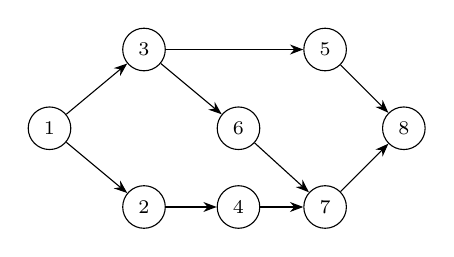
\begin{tikzpicture}
			\begin{scope}[every node/.style={circle,thin,draw}]
 				\node (1) at (0,+0)	{\scriptsize 1};
				\node (2) at (1.2,-1)	{\scriptsize 2};
				\node (3) at (1.2,+1)	{\scriptsize 3};
				\node (4) at (2.4,-1)	{\scriptsize 4};
				\node (5) at (3.5,+1)	{\scriptsize 5};
				\node (6) at (2.4,-0)	{\scriptsize 6};
				\node (7) at (3.5,-1)	{\scriptsize 7};
				\node (8) at (4.5,+0)	{\scriptsize 8};
			\end{scope}

			\begin{scope}[>={Stealth[black]},
				every node/.style={fill=white,circle},
				every edge/.style={draw=black,thin}]
				\path [->] (1) edge (2);				
				\path [->] (1) edge (3);				
				\path [->] (2) edge (4);				
				\path [->] (3) edge (5);				
				\path [->] (3) edge (6);				
				\path [->] (4) edge (7);				
				\path [->] (5) edge (8);				
				\path [->] (6) edge (7);				
				\path [->] (7) edge (8);				
 			\end{scope}
		\end{tikzpicture}
		\subcaption{Example construction plan.}
		\label{fig-house-a}
	\end{subfigure}
	~
	\begin{subfigure}[b]{0.4\textwidth}
		\begin{center}
		    \begin{tabular}{ l l c }
			    & Tasks & Durations (days) \\ \hline
			    1. & Erect walls & 2-4  \\ 
			    2. & Finish walls & 3-5 \\ 
			    3. & Finish roof & 2-6 \\
			    4. & Install plumbing & 3-5 \\
			    5. & Finish exterior & 6-8 \\
			    6. & Install electricity & 3-5 \\
			    7. & Paint interior & 2-4 \\
			    8. & Finishing touches & 1-1 \\
		    \hline
		    \end{tabular}
		\end{center}
	\subcaption{Estimated task durations.}
	\label{fig-house-b}
	\end{subfigure}
	\caption{A motivating example.}
	\label{fig-house}
\end{figure}


This paper addresses a problem which, to our knowledge, has not been addressed in existing literature.
To motivate our problem, let us return to the earlier example and suppose task 7 
(``Paint interior'') is assigned to a painting crew charging \$100 per day.
Assume we are willing to hire them for at least 4 days (the maximum number of days they will need) and for at most 6 days; i.e. we have a budget of \$600 for painting.
With earliest-start dispatching, 7 may start within 8 to 15 days from the project start (the start-date of task 1).
A challenge that arises in this situation is deciding when to hire the painting crew,
because to allow for an expected makespan of a little over 16 days (as mentioned earlier),
we must book the painting crew from the 8-th day and until the 19-th day, at the excessive cost of \$1100.
% ... est requires an agile availability of resources that might be too costly
The solution we examine here, is to use a different dispatching strategy,
associating task 7 with a \emph{planned release-time}, $t_7$, 
before which it may not start even if installing plumbing and electricity are finished earlier than $t_7$.
If we choose that 7 may not start earlier than, e.g., $t_7 = 13$ days from the project start,
we only need to book the painting crew on the 13-th day until the 19-th day, for an acceptable cost of \$600.
However, the price to pay for this stability is an expected makespan increase to a little over 17 days.

Now suppose that after assessing our budget carefully it turns out that each task may deviate at most, say $w$ days, from its respective planned release-time.
The emerging question addressed in this paper is:
\begin{quote}
	Which planned release-times reach the desired level of stability\footnote{As in Bidot et al. \cite{bidot2009}, stability here refers to the extent that a predictive schedule (planned release-times in our case) is expected to remain close to the realized schedule.}
	while minimizing the incurred performance penalty?
\end{quote}

This problem does not involve resource-constraints.
However, task networks are often used in the area of resource-constrained scheduling under uncertainty (see \cite{beck2002,herroelen2005})
to represent solutions (e.g. the \emph{earliest-start policy} \cite{igelmund1983}, the \emph{partial-order schedule} \cite{policella2004,godard2005,bonfietti2014}).
Thus, our work is expected to be useful in dealing with associated problems,
such as distributing slack in a resource-feasible schedule to make it insensitive to durational variability \cite{davenport2014}.

\subsubsection*{Organization}
A formal problem statement and its LP formulation are presented in Section~2. 
As the resulting LP can be quite costly to solve,
Section~3 presents our main result, an efficient dynamic programming algorithm.
Section~4 concludes the paper and outlines issues to be addressed in future work.


	\section{Proactive Stochastic RCPSP}
	\label{sec-problem}
		
	In deterministic and reactive project scheduling,
	the main problem under study (RCPSP and S-RCPSP, respectively) is stated clearly.
	A clearly stated problem model cannot be found in proactive-reactive project scheduling literature,
	perhaps because this research area is still in a burn-in phase.%
	\footnote{Some works refer to \cite{herroelen2004construction} but this is a formal treatment of a
	proactive-reactive \emph{machine} scheduling problem.}%
	Existing literature seems to pursue the general aim 
	of optimizing some tradeoff between expected makespan and 
	expected instability (deviation from the proactive schedule).
	This section presents the formal statement of a proactive-reactive scheduling problem for which
	(heuristic and exact) solution methods are proposed in subsequent sections.
	
	The problem presented here, the Proactive Stochastic RCPSP (PS-RCPSP), 
	asks to find a tuple $(\xE,\xt)$ where $\xE$ is an es-policy and $\xt$ is a proactive schedule,
	minimizing the weighted sum of two performance criteria:
	\begin{enumerate}
		\item expected value of project makespan,
		\item expected value of tardiness with respect to proactive release-times.
	\end{enumerate}
	The first criterion measures lack of robustness and is relevant for obvious reasons.
	The second criterion measures instability and captures the expected 
	deviation of the realized schedule from the proactive schedule.
	Note that $\xt$ prescribes activity release-times (an activity $i$ may not start earlier than $t_i$).
	Intuitively, instability represents the extent to which the proactive start-times can be trusted,
	when used for organizational purposes before and during project execution.
 	
 	An instance of this problem is encoded by a tuple $(n,m,\xq,\xb,E,\xD,\alpha)$.
 	For clarity, we summarize the meaning of problem parameters.
 	Positive integer $n$ is the number of activities and $m$ is the number of resources.
 	Parameters $\xq \in \mathbb{N}^{m\times n}_0$ and $\xb \in \mathbb{N}^m_0$ 
 	define resource requirements and availabilities respectively.
 	Set $E \subseteq \{1,\ldots,n\}^2$ defines pairwise precedence constraints.
 	Stochastic vector $\xD$ is of length $n$ with each element 
 	$D_i$ a stochatic variable (with given distribution $\mathbb{P}[D_i = t]$)
 	which describes the uncertain duration of activity $i$.
 	Finally, parameter $\alpha \in [0,1]$ determines the desired tradeoff between
 	robustness (i.e. minimization of expected makespan) 
 	and stability (i.e. minimization of expected instability).
  	More emphasis can be put on either minimizining makespan (by choosing $\alpha$ closer to one)
  	or minimizing instability (by choosing $\alpha$ closer to zero).
	
 	Formally, the problem can be stated as follows:
 	\begin{align}
 		\min \qquad & f(\xE, \xt) := \alpha \cdot \mathbb{E} \left[ [\xS((\xE,\xt),\xD)]_n \right] + 
 									(1-\alpha) \cdot \mathbb{E} \left[ \sum_{i=1}^n 
 									([\xS((\xE,\xt),\xD)]_i - t_i) \right] 
 									\label{eq-psrcpsp-obj} \\
 		\textrm{s.t.} \qquad	&	\Phi(G(N,\xE)) = \emptyset \label{eq-psrcpsp-1} \\
 								&	T(\xE) \supseteq E \label{eq-psrcpsp-2} \\
 								&	G(N,\xE) \textrm{ is acyclic} \label{eq-psrcpsp-3} \\
 								&	\xE \in \{1,\ldots,n\}^2, \xt \geq 0
 	\end{align}
 	Conditions (\ref{eq-psrcpsp-2},\ref{eq-psrcpsp-3}) ensure there is a non-empty
 	set of schedules satisfying the problem's precedence constraints as prescribed in $E$.
 	Condition (\ref{eq-psrcpsp-1}) ensures that each such schedule also satisfies the
 	problem's resource constraints prescribed by $\xq$ and $\xb$.

\section{Fast computation of planned release-times}
We first show that a fixed relationship between variables $s_{jp}$ and $t_j$
can be assumed while looking for an optimal $(s,t)$.
Based on this, a problem $(P')$ is defined which can be solved instead of $(P)$.

\subsubsection{A tighter formulation}
Begin by rewriting (\ref{P-sjtj}) as $t_j \geq \max_p s_{jp} -w \,, \forall j \in V$.
Now, let $\Lambda$ denote the set of all feasible $(s,t)$ for problem $(P)$ and 
let $\Lambda^* \subseteq \Lambda$ be that part of the solution-space that 
only contains $(s,t)$ for which $t_j = \max_p s_{jp} - w$ for all $j$.

\begin{lemm}
	\label{lemm-Lambda}
	For every feasible $(s,t) \in \Lambda \setminus \Lambda^*$ 
	there exists $(s',t') \in \Lambda^*$ with equal objective value.
\begin{proof}
	Consider feasible $(s,t)$ with
 	$t_j = \max_p s_{j^*p} - w + c$ with  $c > 0$ for some $j^*$.
	Construct $t'$ by letting $t'_j = t_j$ for all $j \neq j^*$ and $t'_{j^*} = t_{j^*} - c = \max_p s_{j^*p} - w$.
	Trivially, if $(s,t)$ is feasible, so is $(s, t')$, with the same objective value.
	Keeping $s$ fixed, we may repeat this construction to enforce that $t_j = \max_p s_{jp} - w$ for all $j$
	and have $(s, t') \in \Lambda^*$.
\end{proof}
\end{lemm}

The previous result allows us to consider the following problem, 
obtained by substituting $\max_{p'\in \z{P}} s_{jp'} - w$ for $t_j$ in $(P)$:
\begin{align}
	\tag{$P'$}
	\min_{s\geq 0} \quad	&	\sum_p s_{np} 								& \\
	\textrm{subject to}\quad	&	s_{jp} \geq s_{ip} + d_{ip}							& (i,j) \in E, p \in \z{P} \label{P'-sisj} \\
				&	s_{jp} \geq \max_{p'\in \z{P}} s_{jp'} - w			& j \in V, p \in \z{P}\label{P'-tjsj} \\
				&	s_{jp} - (\max_{p'\in \z{P}} s_{jp'} -w)  \leq w 	& j \in V, p \in \z{P}\label{P'-sjtj}
\end{align}
Clearly, $(s,t) \in \Lambda^*$ iff $s$ is feasible for $(P')$.%
\footnote{Since  $(s,t)\in \Lambda^*$ implies  $\max_{p'} s_{jp'} - w = t_j$ for all $j$.} 
In other words, the solution-space of $P'$ comprises only those $s$ that can be paired with $t$ by letting $t_j = \max_p s_{jp} - w$
to form a feasible $(s,t)$ for $(P)$.
By Lemma~\ref{lemm-Lambda}, if $s$ is optimal for $(P')$, then $(s,t)$ is optimal for $(P)$.
Also, if $(P)$ has a solution (i.e. if $G(V,E)$ is acyclic),then $(P')$ also has a solution.


\subsubsection{The resulting STP}
Formulation $(P')$ is useful because it can be cast as a certain type of 
Temporal Constraint Satisfaction Problem (TCSP) \cite{dechter1991}.
We start by noting that (\ref{P'-sjtj}) is always true and can be omitted.
Moreover, (\ref{P'-tjsj}) can be rewritten as (\ref{P'-pp}), 
to obtain the following reformulation:
\begin{align}
	\tag{$P'$}
	\min_{s\geq 0} \quad 	&	\sum_p s_{np} 			& \\
	\textrm{subject to} \quad	&	s_{ip} - s_{jp}  \leq -d_{ip}		& (i,j) \in E, p \in \z{P} \label{P'-sisj} \\
				&	s_{jp} - s_{jp'} \leq w			& (p, p') \in \z{P}^2, j \in V \label{P'-pp}
\end{align}

Constraints (\ref{P'-sisj}) and (\ref{P'-pp}) effectively represent the solution-space of a 
Simple Temporal Problem (STP)  \cite{dechter1991} with temporal variables $\{s_{jp}: j\in V, p\in \z{P}\}$.
The structure of the resulting STP (specifically, of its \emph{distance graph} \cite{dechter1991}) is demonstrated in Fig.~\ref{fig-STP}.

\begin{figure}
	\centering
		\begin{subfigure}[b]{0.4\textwidth}
		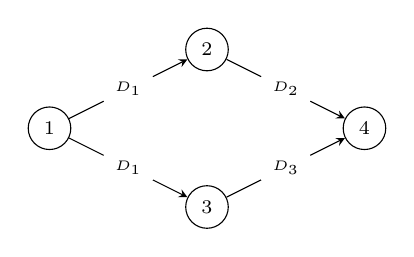
\begin{tikzpicture}
			\begin{scope}[every node/.style={circle,thin,draw}]
				\node (1a) at (+0+0,+0+0)	{\scriptsize $1$};
				\node (2a) at (+2+0,+1+0)	{\scriptsize $2$};
				\node (3a) at (+2+0,-1+0)	{\scriptsize $3$};
				\node (4a) at (+4+0,-0+0)	{\scriptsize $4$};
				
			\end{scope}

			\begin{scope}[>={stealth[black]},
				every node/.style={fill=white,circle},
				every edge/.style={draw=black,thin}]
				\path [->] (1a) edge node {\tiny $D_{1}$} (2a);
				\path [->] (1a) edge node {\tiny $D_{1}$} (3a);
				\path [->] (2a) edge node {\tiny $D_{2}$} (4a);
				\path [->] (3a) edge node {\tiny $D_{3}$} (4a);			
 			\end{scope}
		\end{tikzpicture}
		\subcaption{}
		\label{fig-STN}
	\end{subfigure}
	~
	\begin{subfigure}[b]{0.4\textwidth}
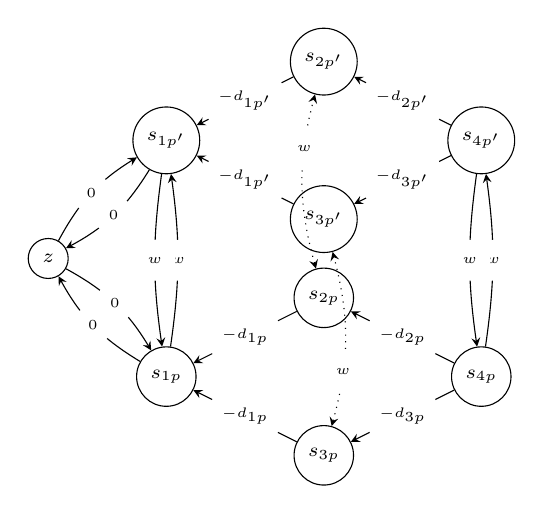
\begin{tikzpicture}
			\begin{scope}[->,>=stealth',shorten >=1pt,auto,
                semithick, scale = 1, transform shape,
                every node/.style={circle,thin,draw}]
				\node (z) at (-1.5,+1.5)	{\scriptsize $z$};
				
				\node (1a) at (+0+0,+0+0)	{\scriptsize $s_{1p}$};
				\node (2a) at (+2+0,+1+0)	{\scriptsize $s_{2p}$};
				\node (3a) at (+2+0,-1+0)	{\scriptsize $s_{3p}$};
				\node (4a) at (+4+0,-0+0)	{\scriptsize $s_{4p}$};
				
				\node (1b) at (+0+0.0,+0+3.0)	{\scriptsize $s_{1p'}$};
				\node (2b) at (+2+0.0,+1+3.0)	{\scriptsize $s_{2p'}$};
				\node (3b) at (+2+0.0,-1+3.0)	{\scriptsize $s_{3p'}$};
				\node (4b) at (+4+0.0,-0+3.0)	{\scriptsize $s_{4p'}$};				
			\end{scope}

			\begin{scope}[>={stealth[black]},
				every node/.style={fill=white,circle},
				every edge/.style={draw=black,thin}]
				
				% z1 arcs
				\path [<-] (z) edge[bend right=15] node {\tiny $0$} (1a);
				\path [->] (z) edge[bend left=15] node {\tiny $0$} (1a);
				\path [<-] (z) edge[bend right=15] node {\tiny $0$} (1b);
				\path [->] (z) edge[bend left=15] node {\tiny $0$} (1b);	
						
				% ij arcs for scenario p
				\path [<-] (1a) edge node {\tiny $-d_{1p}$} (2a);
				\path [<-] (1a) edge node {\tiny $-d_{1p}$} (3a);
				\path [<-] (2a) edge node {\tiny $-d_{2p}$} (4a);
				\path [<-] (3a) edge node {\tiny $-d_{3p}$} (4a);
				
				% ij arcs for scenario p'
				\path [<-] (1b) edge node {\tiny $-d_{1p'}$} (2b);
				\path [<-] (1b) edge node {\tiny $-d_{1p'}$} (3b);
				\path [<-] (2b) edge node {\tiny $-d_{2p'}$} (4b);
				\path [<-] (3b) edge node {\tiny $-d_{3p'}$} (4b);	

							
				% s1p - w - s1p'
				\path [->] (1a) edge[bend right=8] node[] {\tiny $w$} (1b);
				\path [<-] (1a) edge[bend left=8] node[] {\tiny $w$} (1b);
				
				% s2p - w - s2p'
				\path [dotted,<->] (2a) edge[bend left=15] node[pos=0.7] {\tiny $w$} (2b);
				
				% s3p - w - s3p'
				\path [dotted,<->] (3a) edge[bend right=15] node[pos=0.3] {\tiny $w$} (3b);
				
				% s4p - w - s4p'
				\path [->] (4a) edge[bend right=8] node[] {\tiny $w$} (4b);
				\path [<-] (4a) edge[bend left=8] node[] {\tiny $w$} (4b);
			\end{scope}
		\end{tikzpicture}
		\subcaption{}
		\label{fig-STN}
	\end{subfigure}

	\caption{Example task network (a) and resulting STP (b) for a sample $P=\{p, p''\}$.}
	\label{fig-STP}
\end{figure}

The \emph{earliest start time} (est) solution of any given STP (assuming it is consistent)
assigns to each variable the smallest value it may take over the set of feasible solutions.
Therefore,  the est solution of the resulting STP optimally solves $(P')$, leading us to the following observation.

\begin{obsv}
	By Lemma~\ref{lemm-Lambda}, an optimal solution $(s,t)$ for $(P)$ can be formed by finding the 
	earliest start time solution $s$ of the resulting STP and pairing it with $t$ formed by letting 
	$t_j = \max_{p\in \z{P}} s_{jp} - w$ for all $j$.
\end{obsv}

The est value of $s_{jp}$ is the length of the shortest-path (in the distance graph)
from (the node corresponding to) $s_{jp}$ to the special-purpose variable $z$ which is fixed to zero.
Those values can be found with a single-source shortest-path algorithm (e.g. Bellman-Ford \cite{pallottino1984})
in time $O(N M)$ where $N$ is the number of nodes and $M$ the number of arcs. 
In our case, $N=n m$ and $M = O(nm\delta)$, yielding $O(n^3m^2)$; already a better bound than that of solving $(P)$ as an LP.
However, in the following we obtain an even better bound with a dynamic programming algorithm.

\subsubsection{Computing the est solution by dynamic programming}
\begin{algorithm}[!t]
	\caption{Optimal release-times via dynamic programming}
 	\label{alg-main}
	\begin{algorithmic}[1]
		\State $l(s_{1p}) \leftarrow 0$ for all $p\in \z{P}$
		\For{each tier $j$ in a topological sort of $G(V,E)$}
			\State $k_{jp} \leftarrow \min \{l(s_{ip}) - d_{ip}: (i,j)\in E\}$ for all $p\in \z{P}$
			\State $p^* \leftarrow \arg \min \{k_{jp}: p \in \z{P}\}$ 
			\State $l(s_{jp}) \leftarrow \max \{k_{jp}, k_{jp^*} + w\}$ for all $p\in \z{P}$
		\EndFor
		\State $s_{jp} \leftarrow l(s_{jp})$ for all $j\in V, p\in\z{P}$
		\State $t_j \leftarrow \max_{p\in P} s_{jp} - w$ for each $j\in V$ 
	\end{algorithmic}
\end{algorithm}

Let us associate each task $j\in V$ with a corresponding \emph{tier} including all nodes $\{s_{jp}: p \in \z{P}\}$ 
of the STP distance graph.
A few remarks on the structure of the STP are in order.
First, due to (\ref{P'-pp}) the resulting STP is not acyclic, but each cycle only includes nodes that belong to the same tier.
Second, due to (\ref{P'-sisj}) there is a path from each node in tier $j$ to each node in tier $i$ if and only if there is a path from task $i$ to $j$ in $G(V, E)$.

%To form the est solution, we want to compute the shortest-path from each node $s_{jp}$ to special-purpose node $z$.
Let $l(s_{jp})$ denote the shortest-path length from $s_{jp}$ to $z$ (i.e. the value of variable $s_{jp}$ in an optimal solution of $(P')$).
From the structure of the resulting STP, we have:
\begin{align}
	l(s_{jp}) = \min\left\{
		\min_{(i,j)\in E} (l(s_{ip}) - d_{ip}), \min_{p' \neq p} l(s_{jp'}) + w
	\right\}
	\label{def-lsjp}
\end{align}

The existence of cycles complicates solving subproblem $l(s_{jp})$
as it depends on (and is a dependency of) other subproblems $l(s_{jp'})$ in the same tier.
However, we can ``break'' dependencies between subproblems in the same tier as shown below.

Define $k_{jp} := \min_{(i,j)\in E} (l(s_{ip}) - d_{ip})$ and $p^* := \arg \min_{p\in \z{P}} k_{jp}$.
\begin{lemm}
	$l(s_{jp}) = \min\{k_{jp}, k_{jp^*} + w\}$
\begin{proof}
	Begin by noting that the shortest-path from $s_{jp}$ to $z$ visits at most one node $s_{jp'}$ from the same tier.
	As such, for every $s_{jp}$ we have that: either $l(s_{jp}) = k_{jp}$, or $l(s_{jp}) = k_{jp'} + w < k_{jp}$ for some $p' \neq p$.

	Now, note that $l(s_{jp^*}) = k_{jp^*}$,
	since if not (i.e. if $l(s_{jp^*}) \neq k_{jp^*}$),
	then $l(s_{jp^*}) = k_{jp'} + w < k_{jp^*}$ with $p'\neq p^*$, which contradicts the definition of $p^*$.

	Last, we show that if $l(s_{jp}) \neq k_{jp}$ then $l(s_{jp}) = k_{jp^*} + w$.
	Suppose not.
	Since $l(s_{jp}) \neq k_{jp}$ then according to (\ref{def-lsjp}), $l(s_{jp}) = l(s_{jp'}) + w$ but with $p' \neq p^*$.
	Expanding $l(s_{jp'})$ according to (\ref{def-lsjp}),
	\begin{align*}
		\min\{k_{jp'}, \min_{p''\neq p'} l(s_{jp''}) + w\} + w  < l(s_{jp^*}) + w = k_{jp^*} + w
	\end{align*}
	and since $k_{jp'} \geq k_{jp^*}$,
	\begin{align*}
		\min_{p''\neq p'} l(s_{jp''}) + w < k_{jp^*} \\ \Leftrightarrow
		l(s_{jp^*}) + w < k_{jp^*}
	\end{align*}
	which contradicts that $l(s_{jp^*}) = k_{jp^*}$.
\end{proof}
\end{lemm}

The resulting recursion suggests a dynamic programming approach, summarized in Algorithm~\ref{alg-main}.
It involves solving the subproblems of one tier at a time,
visiting tiers according to a topological sort of $G(V,E)$ (recall that tiers correspond to tasks $j\in V$).
Finding a topological sort takes $O(n\delta)$ \cite{tarjan1976},
recalling that $\delta$ denotes the max in-degree of a task in the network.
The overall complexity of Algorithm~\ref{alg-main} is therefore $O(nm\delta) \subseteq O(n^2m)$.

\section{Conclusions and Discussion}

%Given a stochastic task network with $n$ tasks we examined dispatching the tasks as early as possible but not earlier than respective planned release-times.
%Assuming a sample with $m$ realizations of the random task durations vector is given,
%we examined the problem of finding planned release-times that minimize the performance penalty of reaching a desired level of stability.

Given a stochastic task network with $n$ tasks we consider dispatching the tasks as early as possible, subject to (planned) release-times.
Assuming a sample with $m$ realizations of the stochastic durations vector is drawn, we defined an LP for finding 
optimal release-times; i.e. that minimize the performance penalty of reaching a desired level of stability.
%which can be solved at an estimated cost of $O(n^5 m^4)$
%Modern LP solvers can find the optimal with an estimated complexity of $O(n^5 m^4)$, which might be daunting for instances of practical size.
The resulting LP is costly to solve, so
pursuing a more efficient solution method we managed to show that optimal release-times can be expressed 
as a function of the earliest start time solution of an associated Simple Temporal Problem. 
Exploiting the structure of this STP, we were able to define a dynamic programming algorithm 
for finding optimal release-times with considerable efficiency, in time $O(n^2 m)$.

\subsubsection*{Future work}
Since we optimize according to a manageable sample $\z{P}$,
there is a (potentially non-zero) probability $\mathbb{P}_v$ that the realized start-time 
of a task deviates further than $w$ time-units from its planned release-time.
The question of how $\mathbb{P}_v$ (or $\mathbb{E}[\mathbb{P}_v]$ as in \cite{calafiore2005})
depends on $m$ (the size of $\z{P}$) should be addressed in future work.
%
Furthermore, in an earlier paper \cite{mountakis2015}, an LP similar to $(P)$ was used it in a two-step heuristic
for a flavor of the \emph{stochastic resource constrained project scheduling problem} (stochastic RCPSP) \cite{van2008,lamas2015}.
Given a resource allocation determined in a first step, in a second step a LP was used to find planned release-times 
that minimize the total expected deviation of the realized schedule from those release-times.
This heuristic was found to outperform the state-of-the-art in the area of \emph{proactive project scheduling}.
In future work, we shall investigate using the algorithm presented here in order to stabilize the given resource-allocation,
expecting gains in both efficiency and effectiveness.
%
Finally, a potentially related problem, namely PERTCONVG, is studied by Chr{\'e}tienne and Sourd in \cite{chretienne2003},
which involves finding start-times for a task network so as to minimize the sum of convex cost functions.
In fact, their algorithm bears structural similiarities to ours, since subproblems are solved in a topological order.
It would be worth investigating if their analysis can be extended in order to enable
casting the problem studied here as an instance of that problem.


\bibliographystyle{splncs03}
\bibliography{p}

\end{document}
